\documentclass[11pt]{article}
\usepackage[margin=0.85in]{geometry}
\usepackage{parskip}
\usepackage{graphicx}
\usepackage{verbatim}

\title{\vspace{-1.2cm}Module 1 - Q2: MLflow Experiment Comparison}
\author{Name: Kirthan S\\
Roll No.: DA24B009}

\begin{document}
\date{}
\maketitle
\vspace{-0.6cm}


\IfFileExists{comparison.png}{%
\begin{center}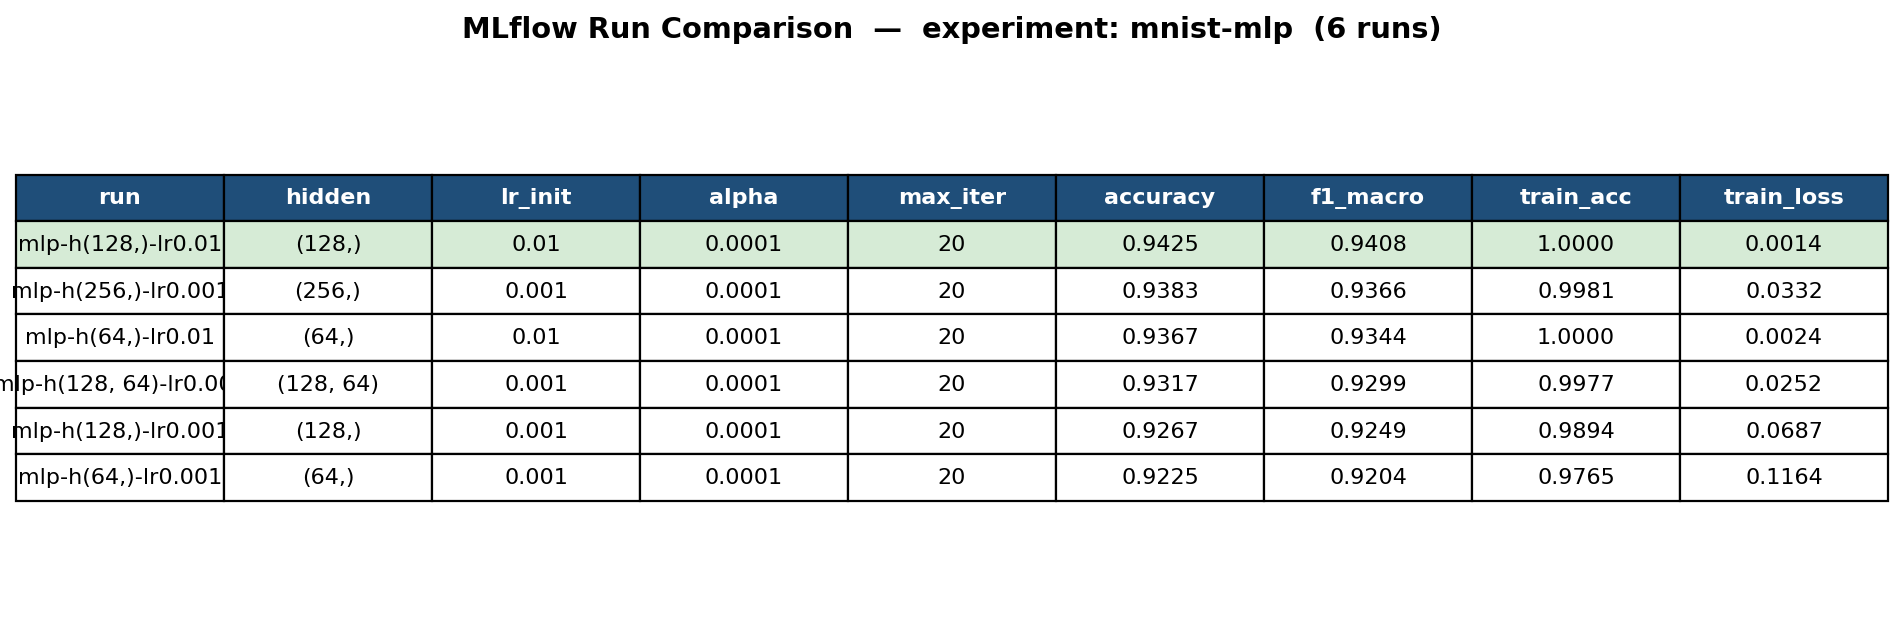
\includegraphics[width=\linewidth]{comparison.png}\end{center}
\vspace{-0.3cm}
}{}

\section*{Analysis}
The best-performing run was run~5 (a single hidden layer of 128 units with
\texttt{learning\_rate\_init}~=~0.01), reaching a test accuracy of 0.9425 and macro-F1 of 0.9408.
Its advantage came almost entirely from the higher learning rate: within the fixed 20-iteration
budget, \texttt{lr}~=~0.01 converged substantially further than 0.001, so the network reached a
better solution before training stopped. Depth did not help --- the two-layer (128,\,64) network
(run~6) scored only 0.9317, below run~5, indicating the extra layer added capacity without benefit
at this data and iteration budget.

Overfitting is clearly visible. For both \texttt{lr}~=~0.01 runs (4 and 5) the training accuracy
reached 1.0000 while test accuracy stayed near 0.94 --- a gap of roughly six percentage points ---
and the logged \texttt{train\_loss} fell close to zero. The model memorises the 4{,}800-sample
training set faster than it generalises, and the gap widens as learning rate and capacity grow.

Of the two swept hyperparameters, \texttt{learning\_rate\_init} had the larger and more consistent
effect: raising it from 0.001 to 0.01 improved test accuracy for both the 64-unit
(0.9225~$\rightarrow$~0.9367) and 128-unit (0.9267~$\rightarrow$~0.9425) networks. Hidden-layer size
helped at the low learning rate (64~$\rightarrow$~256 units: 0.9225~$\rightarrow$~0.9383) but its
effect was smaller and non-monotonic. Learning rate therefore dominated performance.

\section*{Logging code added to the script}
\begin{verbatim}
mlflow.log_param("hidden_layer_sizes", hidden_layer_sizes)
mlflow.log_param("learning_rate_init", learning_rate_init)
mlflow.log_param("alpha", alpha)
mlflow.log_param("max_iter", max_iter)

mlflow.log_metric("accuracy", acc)
mlflow.log_metric("f1_macro", f1)
mlflow.log_metric("train_accuracy", train_acc)
mlflow.log_metric("train_loss", model.loss_)
\end{verbatim}

\end{document}
    